\section{Theoretical framework} 
\label{sec:theoretical_framework}

This section describes basic aspects about terms and elements involved in the problem statement which are also fundamental for a better comprehension of the state of art of this research.

\subsection{Context-aware computing}
\label{sub:context_aware_computing}

Since their introduction to market, mobile devices have evolved from basic cell phones and media players to complex and sophisticated devices like smartphones \cite{Charlesworth2009,Schmidt2011}.
Sensors, advanced wireless communication interfaces and other technological improvements have provided them with more features to be employed in any daily activity.

Furthermore, this set of computing elements have been responsible of the invention of the mobile computing area.
Mobile computing are those computing tasks that can be executed in portable devices while in motion, without losing their computing abilities and accessing to resources at remote locations through wireless networks.
That is, compute tasks anytime and anywhere.

After the invention of mobile computing, the notion of location and context in terms of mobility emerged. 
Location is a simple concept indicating the position of the user in a referenced system. 
The system can be such abstract as the \emph{GPS} or very specific like indoors, e. g. the cafeteria at university campus.

On the other hand, context is a broader and more generic concept.
Oxford dictionary defines concept as:
\begin{quotation}
  The circumstances that form the setting for an event, statement, or idea, and in terms of which it can be fully understood.
\end{quotation}
This definition gives an idea of its abstractness.

Regarding to mobile computing, context still being a non-fully established term.
In \cite{Bellavista2012} several definitions of context are listed:
\begin{itemize}
  \item{Context contains information addressing ``where you are, who you are with, and what resources are nearby'', [Schilit et al. 1994]}.
  \item{Context contains ``any information that can be used to characterize the situation of an entity'', [Dey and Abowd 2000]}.
  \item{Context comprises ``elements for the description of this context information [that] fall into five categories: individually, activity, location, time, and relations'', [Zimmermann et al. 2007]}.
  \item{Context is the ``set of variables that may be of interest for an agent and that influence its actions'', [Bolchini et al. 2009]}.
  \item{Context is ``a four-dimensional space composed of \emph{computing context}, \emph{physical context}, \emph{time context}, and \emph{user context}'', [Chen and Kotz 2000]}.
\end{itemize}

This research considers the latter definition along its development.


\subsection{Mobile sensing apps}
\label{sub:mobile_sensing_apps}

Current trends show there is a large set of applications on which smartphones can be used for. Most of these applications leverage the smartphones’ mobility features and their ability to sense the environment, which turn them into \emph{omni-sensors} \cite{Perez-Torres2012}.

Given the chance to perceive environment, data coming from sensors can be analyzed to detect patterns that represents information about user’s context.
The context then can be used to feedback user with information about his or her activities and adapt smartphone’s behavior accordingly.

As stated, the set of mobile apps that are able to perform tasks related to data collection from sensors and discovering information are called \emph{mobile sensing apps}.

The improvements in data analysis algorithms and similar techniques employed by mobile sensing apps locally at the smartphone and / or in the cloud are increasing the \emph{smartness} of these devices day by day.
In this way, smartphones can get involved in high level logical activities, not only in simple sensor readings or abstract data analysis tasks.

Because of this, the notion of smartphone will be upgraded to \emph{cognitive-phone} \cite{Campbell2012}.
This new class of devices will be able to understand people life patters, reason about their health and well-being and even intervene on their behalf.


\subsubsection{Stages of mobile sensing apps}
\label{sub:stages_of_mobile_sensing_apps}

The duty of mapping raw data into meaningful information for user can become quite complex.
This complexity level depends on the specific characteristics of the sensor being used and the mobile app requirements.

Although the differences in mobile apps and the sensors embedded in mobile devices, some steps are common in their internal functionality.
The list of these steps include the stages of sensor reading, an optional filtering, feature extraction, classification, and post-processing \cite{Ra2012}.
These stages can form a loop, as seen in Figure \ref{fig-mobile-sensing-apps-stages}, that powers up the mobile app.

A basic description of the stages is as follows:
\begin{itemize}
  \item \textbf{Sensor reading:} It includes the request to sensors for reading data from the environment. 
  Common tasks performed in this stage are windowing and framing.

  \item \textbf{Filtering (optional):} In this stage is possible to filter out uninterested data, like outliers or noise.
  Filling data gaps can also be done.
  The purpose of the stage is to prepare a clean and uniform set of data for its use in further steps.

  \item \textbf{Feature extraction:} It performs the extraction of features that helps to discriminate between activities in the classification stage.
  The feature extraction to be employed depends on the type of mobile app being developed.
  The features to be computed can be:
  \begin{itemize}
    \item \emph{Deterministic:} Simple deterministic transformations of raw sensor data, for example frequency content.
    \item \emph{Probabilistic:} Calculated with probability measures, for example the user likelihood of being in a certain location.
  \end{itemize}

  \item \textbf{Classification:} It involves the execution of the mobile app specific classifier.
  Because of the complexity of human activities and the noise existing in sensor data, the classification algorithm are almost always probabilistic, although machine learning techniques have also been used \cite{Choudhury2008}.
  The classifiers can make use of user’s context to improve their performance.

  This stage is the most power consuming one and the execution time may take from seconds up to hours, depending on the data being classified (e. g. in the case of human behavior recognition).
  Because of this, the classifier can be executed locally at the smartphone or in external elements like the cloud.

  \item \textbf{Post-processing:} The classification of data may trigger another loop of continuous sensing-compute chain or other mobile app specific tasks such as displaying feedback to the user or initiating network communication.

\end{itemize}

\begin{figure}
\centering
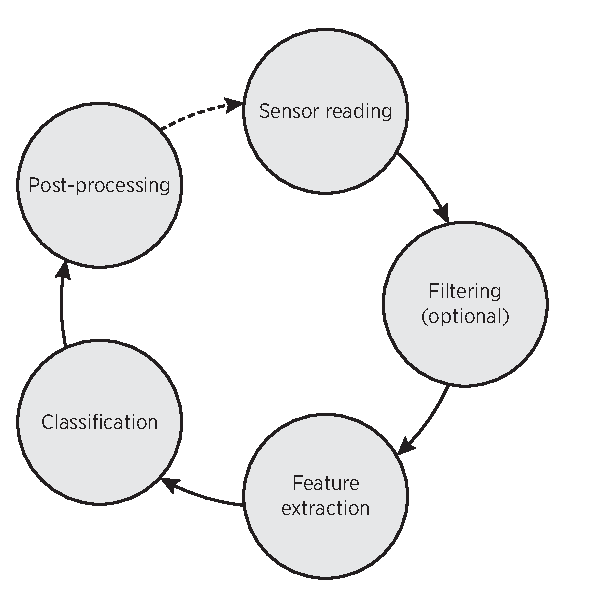
\includegraphics[scale=0.6]{msa-stages}
\caption[Common stages of mobile sensing apps]{Common stages of mobile sensing apps.}
\label{fig-mobile-sensing-apps-stages}
\end{figure}

\subsubsection{Sensing scale of mobile sensing apps}\label{sub:sensing-scale-of-msa}

Depending on the purpose of the mobile app, it may be required to obtain data from one or more users.
The target audience size of the mobile app is known as the \emph{sensing scale}.
There are two sensing scales:
\begin{itemize}
  \item \textbf{Individual sensing scale:} Involves collecting and analyzing data coming from a single person.
  Typically, data refer to track user’s exercise routine and the information is not shared.

  \item \textbf{Community sensing scale:} Involves collecting and analyzing data coming from several users who share a common goal.
  It needs to respond to user specific needs of privacy and anonymity.
  
  This sensing scale is often referred as mobile crowd-sensing and classic examples include traffic monitoring, detection of available parking slots, etc.

  An implicit detail in this sensing scale is the need of a centralized node that acts as a sink of data where analysis processes are executed.
\end{itemize}

This research is conducted targeting the individual sensing scale since the policies to be generated consider analysis of data coming from a single person.


\subsubsection{Paradigms of mobile sensing apps}\label{sub:paradigms-of-msa}

The way how sensors are employed and whether explicit user input is required by a mobile app is known as the \emph{mobile sensing paradigm} \cite{Lane2010}.

There are two sensing paradigms:
\begin{itemize}
  \item \textbf{Opportunistic:} It aims automatic data collection without human participation at all. A remarkable issue of this paradigm is determining the best moment to perform a sensor reading.

  \item \textbf{Participatory:} It leverages the abilities of people requiring their participation to describe the data and to decide the best moment for their capture.

  However, this human dependence can also be a source of errors and noisy data since user is able to upload mislabeled data or even to not to have participation at all.
\end{itemize}


This research is conducted by following the opportunistic paradigm since the smart policies to be generated will decide the duty cycle that sensors must observe, avoiding user participation.


\subsection{Mobile sensing apps examples}
\label{sub:mobile_sensing_apps_examples}

Mobile sensing apps have evolved from apps with specific sensor usage, like using the accelerometer to change the orientation of the screen, to more complex tasks like detecting the user activity e. g. walking, running, climbing stairs, etc.
The usage possibilities offered by mobile sensing apps are high and even increasing after a new sensor is embedded in a smartphone.

In \cite{Wang2012} the \emph{WalkSafe} mobile app is described.
This app improves the safety of pedestrians that walk and talk. WalkSafe leverages the user's context employing the back camera of the smartphone to detect vehicles approaching the user, alerting her or him of a potential unsafe situation.

WalkSafe implements machine learning techniques for detecting the front and back views of moving vehicles.
It employs image recognition algorithms trained off-line with datasets of positive (pictures of front and back views of vehicles) and negative (pictures of side views of vehicles and urban environments) samples producing a set of features for building the car detection model.

Once the model is created, it is uploaded to the phone for its usage in the on-line detection process.
When a phone call is received, the smartphone takes pictures from the back camera, fixes their orientation with accelerometer data, and passed them to the detection module for their processing in real time.
If a car approaching the user is detected, then a vibrating alert is emitted.


Another example of context information usage is \emph{BeWell} \cite{Lane2011a}, which is an app that can monitor and promote some aspects of physical and emotional well-being.
BeWell continuously tracks user behavior along three health dimensions in an \emph{opportunistic} sensing way.

Classifications algorithms are run directly on the phone to infer context information about user's sleep duration, physical activity, and social interaction from sensor data.
BeWell assigns a score to these dimensions and gives a graphical feedback of them to the user.
Sleep duration is inferred by detecting the absence of movement of phone at night.
Physical activity is detected thanks to accelerometer inferring walking, stationary, or running states of the user.
Social interaction is obtained thanks to microphone samples that are used to detect speech or silence time lapses.


A final instance of mobile sensing apps, that employs a \emph{pluggable} sensor via Bluetooth, is \emph{NeuroPhone} \cite{Campbell2010}.
This app works employing neural signals obtained from an electroencephalography (EEG) headset to control smartphones.


Neurophone is a brain-controlled address book dialing app that leverages the generation of P300 \footnote{\emph{P300} is a neuroscience term that refers to a positive peak with a latency of 300 $ms$ that is elicited when brain concentrates on a task specific stimulus among a pool of stimulus.} signals in human brain.
The smartphone shows a sequence of pictures of address book contacts and a potential P300 brain is elicited when a photo matches the person whom the user wishes to call.
The data generated by the EEG headset is transmitted to the smartphone, on which a classification process detects an actual P300 and triggers the contact’s phone number dialing.

% \subsubsection{Convergence of sensing applications into the IoT}
% % Mention that smart devices are connecting people, globally and that is the final objective of them.
% Mobile sensing apps are contributing to the adoption of mobile devices by society.
% By leveraging the communication facilities (for instance, the Internet enabled feature) of smart devices, the vision of future world is one such people will be globally connected with others anywhere and anytime.

% % Mention that a fully connected world has been spotted in other scenarios.
% This vision of a fully connected world has been also chased in other scenarios, like the industry, where the items to be connected are common real world objects like tools, machines, buildings, vehicles, etc.
% % Introduce the smart objects
% Such items are enhanced with an identification mechanism like RFID and basic computation, sensing, and communication facilities that turn them into smart objects \cite{Kortuem2010}.
% % Mention that when 2+ smart objects communicate, then there is a M2M
% Thanks to these enhanced capabilities, the smart objects are able to collect data of their environment and interact with other smart objects, creating a M2M communication system.

% % Introduce the objectives of M2M
% M2M communication systems aim to go beyond the industrial environment and be the base mechanism to query and deliver data between any objects of the real world.
% Such communication should be allowed in any direction, from object A to object B and vice versa.
% Thanks to this, it will be possible to collect data from sensors of a smart object or to instruct an object to behave in a particular way, modifying its environment.

% % Mention that the sets SP-MSA and SO-M2M are similar but also present differences.
% The sets conformed by smartphone--mobile sensing apps and smart objects--M2M target different scenarios but share several features shown in Table \ref{tbl:msa-vs-m2m}.
% The only aspects they do not share are the \emph{communicates with} and application purpose.
% \emph{Communicates with} refers to the type of entity a smartphone or a smart object establish communication with.
% Typically a smart object will communicate always with other smart objects, like in any M2M communication system instance.
% On the other hand, a smartphone can communicate with other objects but also with humans.
% It means that smart devices, like the smartphone, offer several interaction ways for communicating with people while smart objects do not.

% The application purpose marks another difference between smartphones and smart objects.
% A smart object has a specific purpose: it only performs a single or a reduced set of tasks, it is not designed to execute third party apps; indeed, the concept of a mobile OS is out of its scope.
% In change, a smartphone is a general purpose item that can be employed in a wide range of applications. Smart devices include a mobile OS that makes it possible to install third party apps and expand their functionality.
% Broadly speaking, a smart device, like a smartphone, can be considered a smart object but this relationship does not apply inversely.

% \begin{table}
%   \centering
%     \scriptsize
%     \begin{tabularx}{0.70\linewidth}{ccc}
%       \toprule
%       \textbf{Feature} & \textbf{Smartphone} & \textbf{Smart object} \tabularnewline
%       \midrule
%         \textbf{Context awareness} & Yes (Through sensors) & Yes (Through sensors) \tabularnewline
%         \textbf{Communication} & Yes (Wireless) & Yes (Wired, Wireless) \tabularnewline
%         \textbf{Processor} & Yes (Multi-core) & Yes (Low power consuming) \tabularnewline
%         \textbf{Storage} & Yes (In the order of Gigabytes) & Yes (reduced size) \tabularnewline
%         \textbf{\emph{Communicates with}} & Human, other objects & Other objects (machines) \tabularnewline
%         \textbf{Purpose} & General & Specific \tabularnewline
%       \bottomrule
%     \end{tabularx}
   
%     \caption{Comparison of the characteristics of smartphones versus smart objects}
%     \label{tbl:msa-vs-m2m}
% \end{table}

% In any case, the sets smartphone--mobile sensing apps and smart objects--M2M can be abstracted as systems that interconnect \emph{things} in an evolved vision of Internet known as the IoT.
% % Tell a brief IoT interaction-flow
% In the IoT every real world object has a virtual representation and can understand its environment and role in a particular activity, trigger special actions when certain events occur and materialize these actions in both physical and virtual worlds \cite{Uckelmann2011}.
% If mobile computing has the dimension of time and place, IoT adds the new dimension of thing (see Figure \ref{fig-iot-dimensions}).
% Summarizing: IoT aims to produce a fully connected world with unlimited application systems that address any real world problem.

% \begin{figure}
% \centering
% 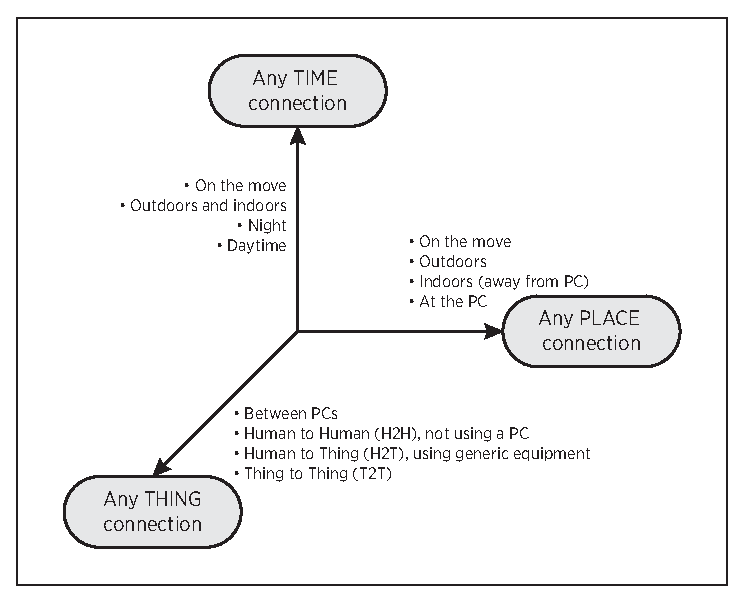
\includegraphics[scale=0.6]{iot-dimensions}
% \caption[Dimensions of the IoT]{Dimensions of the Internet of Things: time, place, thing.}
% \label{fig-iot-dimensions}
% \end{figure}